\section{Экспериментальная часть}
\label{cha:research}

В данном разделе будут приведены примеры работы разработанной программы и поставлен эксперимент по сравнению производительности
в зависимости от сложности моделируемой сцены. Сложность оценивается количеством используемых на сцене поверхностей.

\subsection{Результаты разработки}

\subsubsection{Описание интерфейса}

В верхнем правом углу программы располагается панель управления, позволяющая контролировать созданные объекты, например, вращать их, масштабировать или перемещать (пример такой панели для куба, сферы и цилиндра привелён на рисунке \ref{fig:panel}). 
\begin{figure}[h]
	\centering
	\captionsetup{justification=centering}
	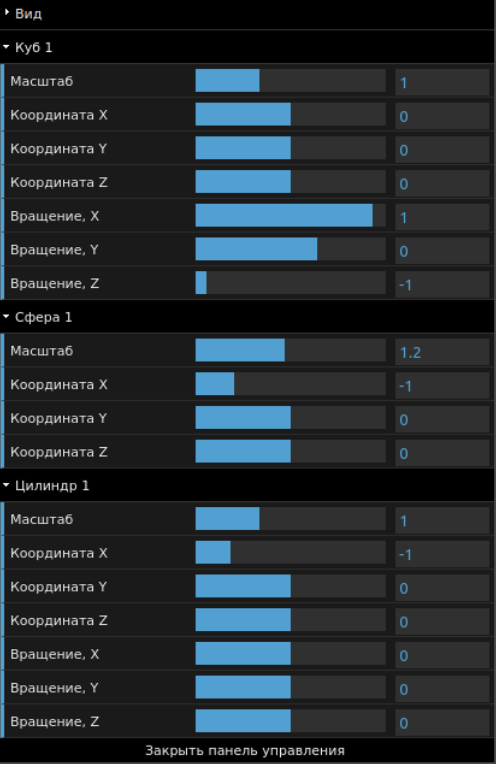
\includegraphics[width=50mm]{img/panel.png}
	\caption{Пример панели управления для куба, сферы и цилиндра}
	\label{fig:panel}
\end{figure}

В нижнем правом углу располагаются кнопки, позволяющие пользователю перейти к созданию нового объекта или к удалению последнего созданного (рисунок \ref{fig:add-buttons}).
\begin{figure}[h]
	\centering
	\captionsetup{justification=centering}
	
\includegraphics[width=90mm]{img/add-buttons.png}
	\caption{Кнопки добавления нового объекта и удаления последнего созданного}
	\label{fig:add-buttons}
\end{figure}

Разработанная программа позволяет пользователю создавать твердотельные модели на основе примитивов (куб, цилиндр, сфера и тор) и использовать логические операции (объединение, пересечение, вычитание). Присутствует возможность добавлять на сцену объекты, удалять их и преобразовывать, а также менять позицию камеры.

\subsubsection{Демонстрация работы программы}

На рисунке \ref{fig:example-1} продемонстрирована рабоота программы на примере вычитания куба из сферы и объединения с цилиндром.

\begin{figure}[h]
	\centering
	\captionsetup{justification=centering}
	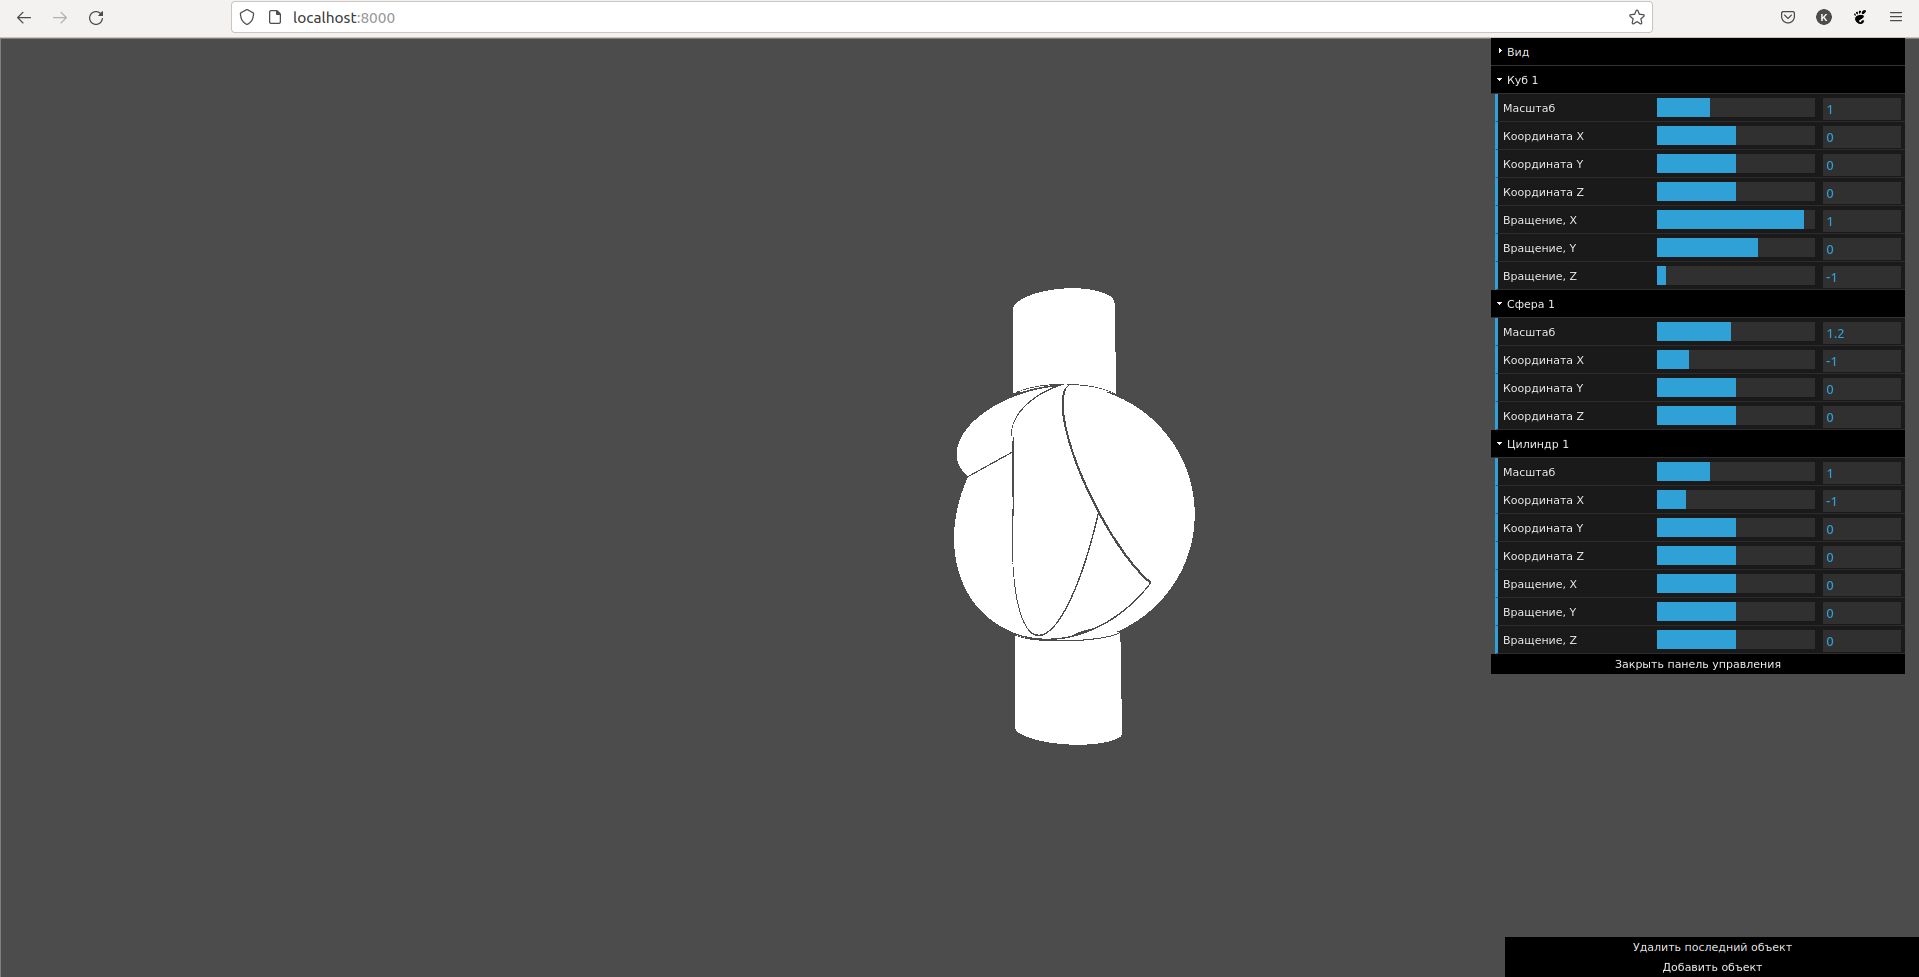
\includegraphics[width=138mm]{img/example-1.png}
	\caption{Демонстрация  работы  программы  (композиция  моделей 
		куба, сферы и цилиндра)}
	\label{fig:example-1}
\end{figure}
\clearpage

На рисунке \ref{fig:example-2} продемонстрирована работа программы на примере пересечения куба с тором и объединения с цилиндром.

\begin{figure}[h]
	\centering
	\captionsetup{justification=centering}
	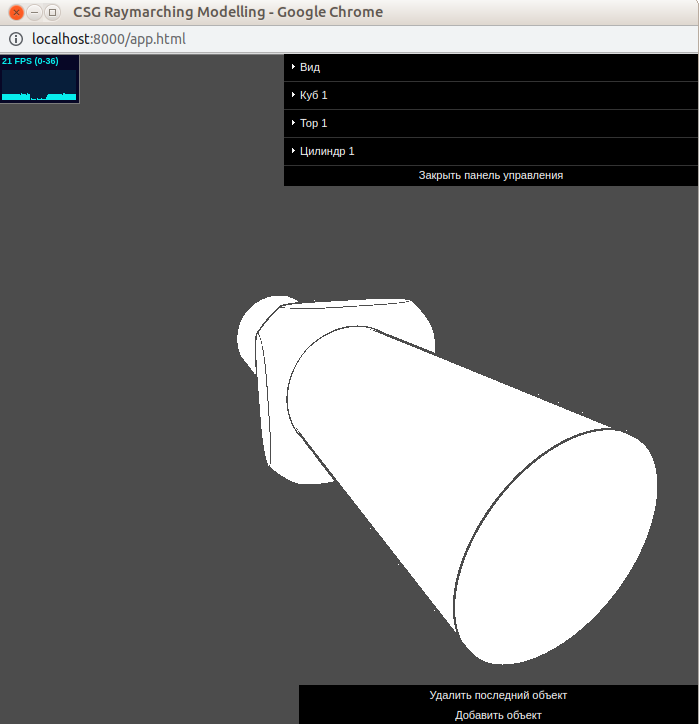
\includegraphics[width=140mm]{img/example-2.png}
	\caption{Демонстрация  работы  программы  (композиция  моделей 
		куба, тора и цилиндра)}
	\label{fig:example-2}
\end{figure}

\subsection{Постановка эксперимента}

Целью эксперимента является сравнение производительности приложения при использовании встроенной и 
дискретной видеокарт.
Производительность будет оцениваться с помощью измерения количества кадров в секунду (FPS), с которами работает приложение.
Нагрузка будет меняться в зависимости от количества объектов, расположенных на сцене.  

\clearpage


Технические характеристики устройства, на котором выполнялось тестирование:

\begin{itemize}[label=---]
	\item Операционная система: Ubuntu 21.04 \cite{ubuntu} 64-bit;
	\item Память: 16 Гб;
	\item Процессор: Intel Core™ i5-8300H \cite{intel} с тактовой частотой  2.30 ГГц;
	\item Видеокарты: 
	\subitem--- AMD Radeon (TM) VEGA 8 Graphics (встроенная) \cite{amd-graphics};
	\subitem--- NVIDIA GeForce GTX 1080 (дискретная) \cite{nvidia-graphics}.
\end{itemize}

Тестирование проводилось на ноутбуке, включенном в сеть электропитания. Во время тестирования ноутбук был нагружен только системой тестирования (работающим приложением) и системным окружением операционной системы.

\subsection{Сравнение производительности}

Результаты сравнения производительности сцен разной нагруженности приведены в таблице \ref{tb:comp_fps}.
\begin{table}[h]
	\caption{Сравнение FPS при запуске приложения на встроенной и дискретной видеокартах.}
	\begin{tabular}{|l|l|l|}
		\hline
		Количество объектов & FPS-NVIDIA & FPS-AMD \\
		\hline
		1                   & 60         & 24        \\
		2                   & 55         & 18        \\
		3                   & 48         & 10        \\
		4                   & 36         & 8        \\
		5                   & 32         & 6         \\
		\hline
	\end{tabular}
	\label{tb:comp_fps}
\end{table}

\clearpage

Результаты тестирования приводят к следующим выводам:
\begin{enumerate}[label=\arabic*)]
	\item с ростом количества объектов, количество FPS уменьшается (в лучшем случае 60 кадров (24 на встроенной), в худшем 32 кадра (6 на встроенной));
	\item дискретная видеокарта позволяет получить большее количество кадров, которое приемлемо для использования приложения в режиме реального времени (30+ FPS),
	это объясняется наличием встроенной памяти (2 ГБ) и большей мощностью в сравнении с встроенной, которая менее производительна, а также использует разделяемую память (часть оперативной);
	\item встроенной видеокарты недостаточно для выполнения программы в режиме реального времени - приемлемое FPS должно быть около 30 и более, встроенная 
	(в лучшем случае - 1 объект на сцене) позволяет получить лишь 24 FPS ---  для режима реального времени недостаточно;
	\item в среднем дискретная видеокарты производительнее встроенной в 4 раза.
\end{enumerate}


